% arara: latex: { interaction: nonstopmode, options: ['-halt-on-error'] }
% arara: dvisvgm: { options: ['--no-fonts', '--exact-bbox', '--zoom=-1'] }
% These are diagrams in CENTER space, not enclosing disks in input space.
% Fixed boundary point P=(0,0). Every input x induces 2u.x >= |x|^2.
% Left inputs: (2,0), (1,1/2). Their half-planes are
% u_x >= 1 and u_x + u_y/2 >= 5/8; the projection is (1,0).
% Right inputs: (2,0), (0,2), (1,1). Their half-planes are
% u_x >= 1, u_y >= 1, and u_x+u_y >= 1; the projection is (1,1).
\documentclass[tikz,border=8pt,11pt]{standalone}
\usepackage{amsmath,amssymb}
\definecolor{circleblue}{HTML}{0072B2}
\definecolor{pointred}{HTML}{D55E00}
\definecolor{fixedpurple}{HTML}{8B4C9D}
\definecolor{ink}{HTML}{25313C}
\definecolor{muted}{HTML}{7C8792}
\tikzset{
  active/.style={draw=fixedpurple,line width=1.2pt},
  inactive/.style={draw=muted,line width=0.85pt},
  level/.style={draw=circleblue,dashed,line width=0.9pt},
}
\newcommand{\axes}{%
  \draw[->,ink!60] (-1.6,0) -- (3.3,0) node[right] {$u_x$};
  \draw[->,ink!60] (0,-1.6) -- (0,2.8) node[above] {$u_y$};
  \fill[ink] (0,0) circle[radius=2.3pt];
  \node[below left,inner sep=4pt] at (0,0) {$P=0$};
}
\begin{document}
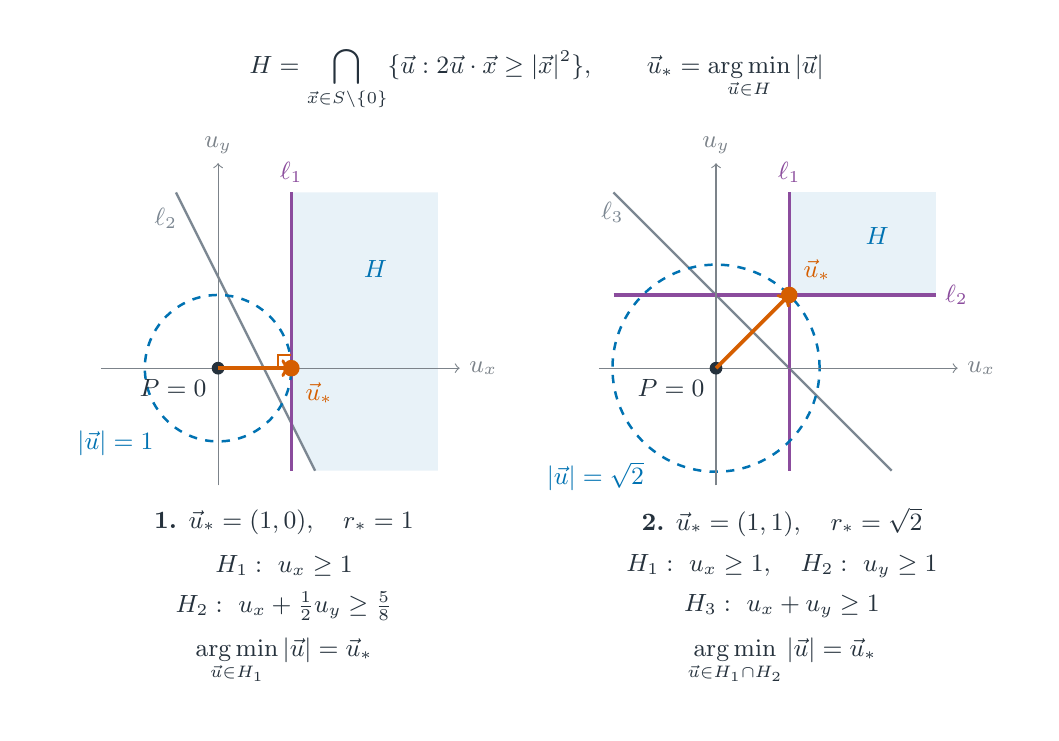
\begin{tikzpicture}[x=0.93cm,y=0.93cm,font=\small,text=ink]
  \fill[white] (-2.6,-4.7) rectangle (11.1,4.65);
  \node at (4.35,3.95) {$H=\displaystyle\bigcap_{\vec x\in S\setminus\{0\}}\{\vec u:2\vec u\cdot\vec x\ge|\vec x|^2\},
    \qquad \vec u_*=\underset{\vec u\in H}{\operatorname{arg\,min}}\,|\vec u|$};

  \begin{scope}
    \fill[circleblue!9] (1,-0.75) -- (1,2.4) -- (3,2.4)
      -- (3,-1.4) -- (1.325,-1.4) -- cycle;
    \draw[inactive] (-0.575,2.4) -- (1.325,-1.4);
    \draw[active] (1,-1.4) -- (1,2.4);
    \draw[level] (0,0) circle[radius=1];
    \axes
    \draw[->,pointred,line width=1.3pt] (0,0) -- (1,0);
    \fill[pointred] (1,0) circle[radius=3pt];
    \node[below right,text=pointred,inner sep=5pt] at (1,0) {$\vec u_*$};
    \draw[pointred,line width=0.7pt] (0.82,0) -- (0.82,0.18) -- (1,0.18);
    \node[text=fixedpurple,above] at (1,2.4) {$\ell_1$};
    \node[text=muted,left] at (-0.43,2.05) {$\ell_2$};
    \node[text=circleblue] at (2.15,1.35) {$H$};
    \node[text=circleblue,below left] at (-0.75,-0.72) {$|\vec u|=1$};
    \node at (0.9,-2.1) {\textbf{1.} $\vec u_*=(1,0),\quad r_*=1$};
    \node at (0.9,-2.7) {$H_1:\ u_x\ge1$};
    \node at (0.9,-3.25) {$H_2:\ u_x+\tfrac12u_y\ge\tfrac58$};
    \node at (0.9,-4) {$\underset{\vec u\in H_1}{\operatorname{arg\,min}}\,|\vec u|=\vec u_*$};
  \end{scope}

  \begin{scope}[xshift=6.324cm]
    \fill[circleblue!9] (1,1) rectangle (3,2.4);
    \draw[inactive] (-1.4,2.4) -- (2.4,-1.4);
    \draw[active] (1,-1.4) -- (1,2.4);
    \draw[active] (-1.4,1) -- (3,1);
    \draw[level] (0,0) circle[radius={sqrt(2)}];
    \axes
    \draw[->,pointred,line width=1.3pt] (0,0) -- (1,1);
    \fill[pointred] (1,1) circle[radius=3pt];
    \node[above right,text=pointred,inner sep=5pt] at (1,1) {$\vec u_*$};
    \node[text=fixedpurple,above] at (1,2.4) {$\ell_1$};
    \node[text=fixedpurple,right] at (3,1) {$\ell_2$};
    \node[text=muted,left] at (-1.13,2.13) {$\ell_3$};
    \node[text=circleblue] at (2.2,1.8) {$H$};
    \node[text=circleblue,below left] at (-0.85,-1.15) {$|\vec u|=\sqrt2$};
    \node at (0.9,-2.1) {\textbf{2.} $\vec u_*=(1,1),\quad r_*=\sqrt2$};
    \node at (0.9,-2.7) {$H_1:\ u_x\ge1,\quad H_2:\ u_y\ge1$};
    \node at (0.9,-3.25) {$H_3:\ u_x+u_y\ge1$};
    \node at (0.9,-4) {$\underset{\vec u\in H_1\cap H_2}{\operatorname{arg\,min}}\,|\vec u|=\vec u_*$};
  \end{scope}
\end{tikzpicture}
\end{document}
